\documentclass[sigconf]{acmart}

%\usepackage{booktabs} % For formal tables
\usepackage{gensymb}


% Copyright
%\setcopyright{none}
%\setcopyright{acmcopyright}
%\setcopyright{acmlicensed}
\setcopyright{rightsretained}
%\setcopyright{usgov}
%\setcopyright{usgovmixed}
%\setcopyright{cagov}
%\setcopyright{cagovmixed}


% DOI
\acmDOI{10.475/123_4}

% ISBN
\acmISBN{123-4567-24-567/08/06}

%Conference
\acmConference[EMSOFT'18]{ACM International Conference on Embedded Software}{October 2018}{Turin, Italy}
\acmYear{2018}
\copyrightyear{2018}


\acmArticle{1}
\acmPrice{15.00}

% These commands are optional
%\acmBooktitle{Transactions of the ACM Woodstock conference}
%\editor{Jennifer B. Sartor}
%\editor{Theo D'Hondt}
%\editor{Wolfgang De Meuter}


\begin{document}
\title{Work-in-Progress: Hierarchical Control of a Catoptric Surface}
%\titlenote{Produces the permission block, and
 % copyright information}
%\subtitle{Work-in-Progress}


\author{Roger D. Chamberlain, Chandler Ahrens, Chris Gill, and Scott A. Mitchell}
%\author{Anonymous for review}
\affiliation{%
  \institution{Washington University in St. Louis}
%  \institution{[Institution redacted]}
%  \streetaddress{One Brookings Dr.}
%  \city{Dublin}
%  \state{Ohio}
%  \postcode{43017-6221}
}
\email{{roger,cahrens,cdgill,scott.a.mitchell}@wustl.edu}
%\email{[Email]}


% The default list of authors is too long for headers.
\renewcommand{\shortauthors}{R. Chamberlain et al.}
%\renewcommand{\shortauthors}{Anonymous for review}


\begin{abstract}
The control of a catoptric (mirror-based) surface is decomposed
hierarchically. The positioning control of individual mirrors
is handled by low-level controllers for each drive motor, and the
overall control decisions are guided by a Markov decision process.
\end{abstract}

%
% The code below should be generated by the tool at
% http://dl.acm.org/ccs.cfm
% Please copy and paste the code instead of the example below.
%
\begin{CCSXML}
<ccs2012>
<concept>
<concept_id>10011007.10010940.10010971.10010564</concept_id>
<concept_desc>Software and its engineering~Embedded software</concept_desc>
<concept_significance>500</concept_significance>
</concept>
</ccs2012>
\end{CCSXML}

\ccsdesc[500]{Software and its engineering~Embedded software}


\keywords{Catoptric systems, hierarchical control, Markov decision process (MDP), daylighting systems}


\maketitle

\section{Introduction}
\label{sec:intro}

Daylighting, the use of natural light for illumination, is clearly
beneficial in human-occupied
spaces~\cite{hhm15,Leslie03}.
Yet, daylighting design is dominated by passive window positioning
and configuation~\cite{Leslie03} rather than active control mechanisms,
except in a few cases~\cite{kt16}.

To explore the possibilities of actively controlled daylighting systems,
a catoptric (mirror-based) surface has recently been installed in
the south facing glass fa\c cade of a campus building
(see Figure~\ref{fig:steinberg})~\cite{acadia18}.
The catoptric surface is comprised of 650 mirrors, each with 2 independent
degrees of freedom (pan and tilt), providing a range of motion of
approximately a full hemisphere.

With 256 possible positions per degree of freedom (180\degree{} range
and 0.7\degree{} resolution), 2 degrees of freedom per mirror, and 650 mirrors, 
there are over 300,000 possible stable configurations of the catoptric surface.
Add to this the desire to control mirror movement profiles (i.e.,
acceleration), and the number of configurations grows considerably.

In this paper, we describe our approach to controlling the catoptric surface.
The control is decomposed hierarchically, with low-level controllers
handling individual mirror motions and high-level control managing the
desired position (and movement profiles) of the set of mirrors.

\begin{figure}[ht]
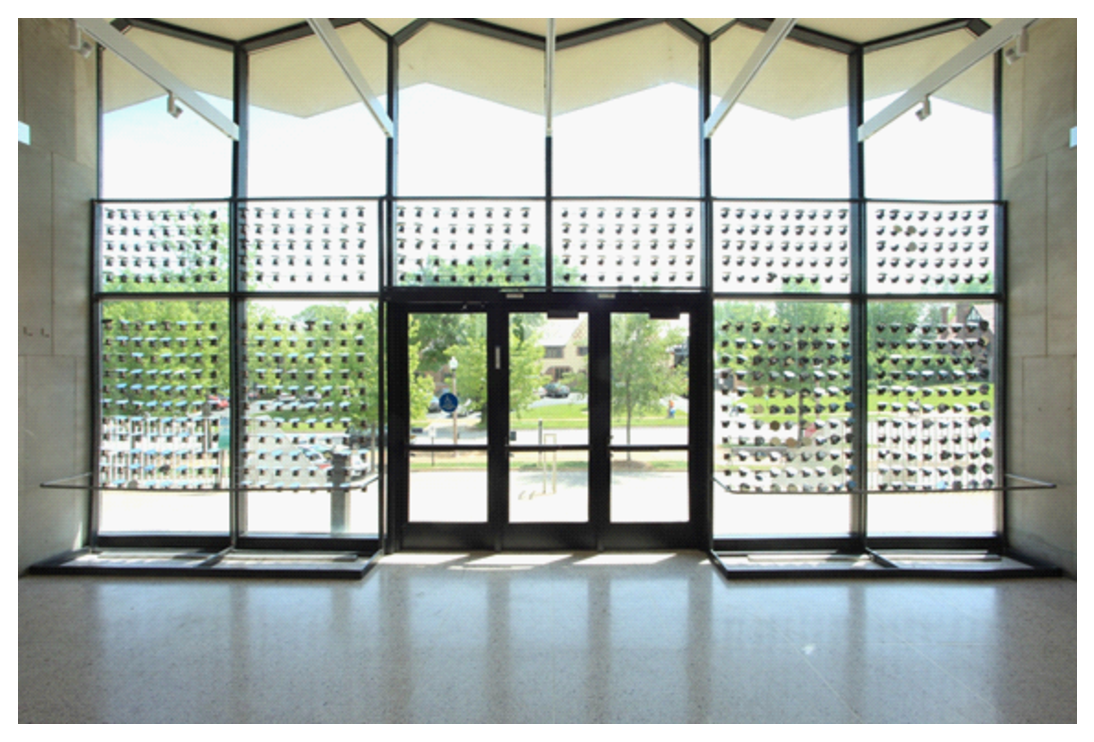
\includegraphics[width=0.92\columnwidth]{steinberg}
\caption{Array of mirror units inside of a south-facing glass fa\c cade~\protect\cite{acadia18}.}
\label{fig:steinberg}
\end{figure}



\section{Individual Mirror Control}
\label{sec:mirror}

The pan and tilt of each mirror unit is driven by a pair of
unipolar 12V stepper motors, commanded over an I2C bus by an
Arduino Uno\footnote{\url{https://www.arduino.cc}} on either end of
each row of mirrors (see Figure~\ref{fig:mirror})~\cite{acadia18}.
The two halves (east and west) have a
Raspberry~Pi\footnote{\url{https://www.raspberrypi.org}}
communicating with the Arduino Unos over USB, which also provides
wireless connectivity to a remote PC running Rhino3D/Grasshopper.

\begin{figure}[ht]
\centering
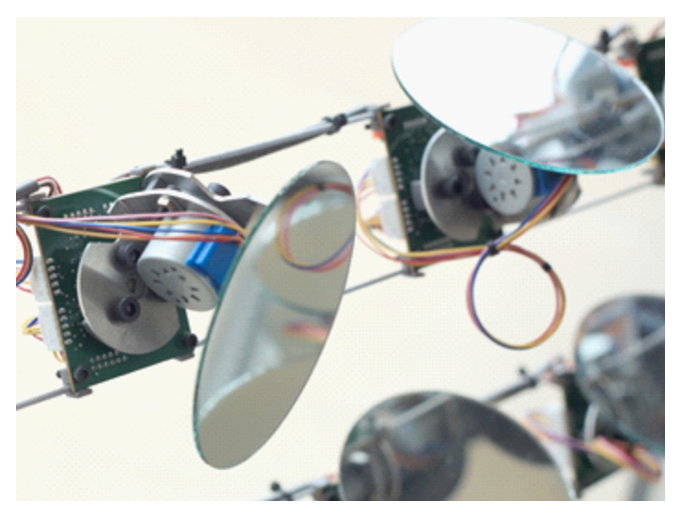
\includegraphics[width=0.98\columnwidth]{mirror}
\caption{Individual mirror units,
each with pan and tilt control~\protect\cite{acadia18}.}
\label{fig:mirror}
\end{figure}

The stepper motors are running open loop,
(i.e., there are no shaft encoders in the system),
so to establish known position each
motor is driven to the physical stops (a reset position) and then
the Arduino Unos accept motor movement commands that include
mirror ID ($x$ and $y$ position in the surface), which motor (pan vs.\ tilt),
direction, and number of steps.
The local Arduino Unos make no
attempt to retain position information, that is the responsibility
of the higher-level system.

To enable movement profiles, we will extend the messaging protocol
and use the Arduino Unos to provide more nuanced timing in their
motor movement commands. This is fairly straightforward in a stepper
motor-driven system, in which individual step control is available.

The resulting catoptric surface is effectively an IoT device, which
relies on network connectivity for high-level control.

\section{Global Mirror Control}
\label{sec:mdp}

We are investigating the use of Markov Decision Processes (MDPs) to
implement the high-level control of which mirror should be in what position.
MDPs represent a general approach to modeling optimization
problems and have been applied to a diverse set of
application areas. Examples include: robotics~\cite{ab10},
%economics~\cite{bs98}, % experiment design~\cite{White93},
medical decisions~\cite{ahsr10}, manufacturing~\cite{yyl04},
agriculture~\cite{Kristensen03},
real-time scheduling~\cite{gtsg08},
and wireless spectrum management~\cite{mgc16}.

Here, we adopt the definition of Glaubius et al.~\cite{gtsg08}
of a (discrete-time) MDP as a 5-tuple
$(\mathcal{X}, \mathcal{A}, T, R, \gamma)$, with \emph{states}
$\chi \in \mathcal{X}$, \emph{actions} $a \in \mathcal{A}$,
and a transition system, $T$, which gives probability
$P_T (\chi' \mid \chi, a)$ of transitioning from state $\chi$ to
state $\chi'$ on action $a$.
The reward function $R(\chi, a, \chi') \in \mathbb R_{\ge 0}$ describes the
reward that accrues when transitioning from state $\chi$ to
state $\chi'$ via action $a$, under a discount factor, $\gamma$,
to ensure convergence of the long term reward.

For a catoptric surface with $N_m$ motors, each of which has $N_s$
steps, we define a state to be a vector of $N_m$ motor positions,
each of which has a value between 0 and $N_s$.  This is illustrated
for a single-mirror, 2-motor (pan and tilt) surface in Figure~\ref{fig:mdp2}.
The transitions represent single steps for the drive motors.
Self-loops (not shown) would represent no motion.  In the figure,
only one motor at a time is allowed to be in motion.  To support simultaneous
motion, diagonal transitions would be added to the transition system, $T$.
The figure generalizes to additional mirrors by adding two
additional dimensions per mirror.

\begin{figure}[ht]
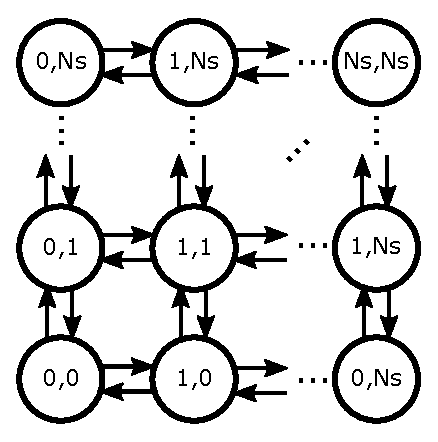
\includegraphics[width=0.5\columnwidth]{mdp2}
\caption{Single-mirror, 2-motor MDP state space and associated transitions.
Horizontal transitions represent moving the pan motor and vertical transitions
represent moving the tilt motor.}
\label{fig:mdp2}
\end{figure}

We define the reward function, $R$, as having multiple components. First,
it incorporates the match of the realized illumination pattern with a
desired illumination pattern (using ray-tracing~\cite{acadia18}).
Second, it includes a measure of the impact
of mirror motion on the reliability of the mirror assemblies. Third, it
factors in the current positioning uncertainty due to running the
motors open loop (i.e., low uncertainty at the range limit, growing
uncertainty with each movement).

MDP theory assures us that there exists a policy (choice
of action, $a$, in each state, $\chi$) that maximizes the expected reward.
While this policy is, in general, exponentially expensive
to compute, we are exploring heuristics that closely match the optimal
policy and are more computationally feasible in real time (so as to quickly
accommodate changes in sun position, desired illumination pattern, etc.).

\section{Conclusions}
\label{sec:conclude}

The current state of the system is as follows:
the physical installation is complete,
the individual motor control software is complete and operational,
and a number of variations on the global control MDP are being investigated.
Extensions to the MDP that we are
considering include: multiple motors in simultaneous motion, multi-step
transitions that include acceleration profiles, and model reduction
techniques to diminish the inevitable state-space explosion.


\section*{Acknowledgements}
This work is supported by the Washington Univ.~Int'l Center for
Energy, Environment and Sustainability (InCEES).

\bibliographystyle{ACM-Reference-Format}
\bibliography{paper}

\end{document}
